\chapter{Xây dựng API xử lý}

\section{Tổng hợp và chuẩn hóa ngân hàng câu hỏi chương Xác suất – Thống kê lớp 11}
Phần này tiến hành tổng hợp và chuẩn hóa ngân hàng câu hỏi trắc nghiệm chương Xác suất – Thống kê lớp 11 dựa trên 03 nội dung cơ bản trong SGK Đại số và giải tích 11 (ban cơ bản): Quy tắc đếm, hoán vị, tổ hợp, chỉnh hợp (bài 1, 2), nhị thức Newton (bài 3) và xác suất của biến cố (bài 4, 5).\par
Để sử dụng được ngân hàng câu hỏi cho việc đánh giá riêng lẻ từng học sinh theo \textit{lý thuyết ứng đáp} câu hỏi (IRT), cần có một ngân hàng câu hỏi đã chuẩn hóa sẵn theo các tham số \textit{độ khó} ($b$) và \textit{độ phân biệt} ($a$) – là những tham số độc lập so với mẫu. Phần lớn các câu hỏi trong luận văn này được tổng hợp từ \cite{luyen2018xay} và \cite{truc2018xay}. Trong đó có 44 câu hỏi có thể sử dụng ngay (đã được thực nghiệm và phân tích bằng IATA):\par
\noindent\textbf{Câu hỏi trắc nghiệm phần Quy tắc đếm, hoán vị, tổ hợp, chỉnh hợp \cite{truc2018xay}:}\par
\begin{enumerate}[label=\textbf{Câu \arabic*.},align=left,left=0cm..0cm,itemindent=*]
	% Quy tắc đếm
	\item Mỗi ngày T đều đi từ nhà (vị trí $A$) tới trường (vị trí $D$) được nối với nhau như hình vẽ bên dưới. T có bao nhiêu con đường có thể đi và không đi qua một vị trí 2 lần?\par {\centering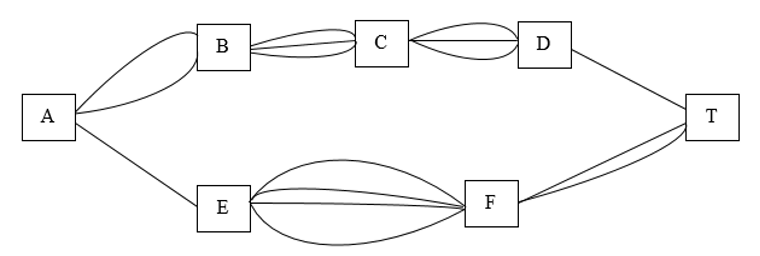
\includegraphics[width=9cm]{G1-Q9.png}\par}
	\begin{enumerate}[label=\textbf{\Alph*.},align=left,left=1cm..0cm,itemindent=*]
		\item $26$. \item $144$. \item $16$. \item $63$.
	\end{enumerate}
	\item Kỷ niệm 77 năm ngày thành lập Đoàn TNCS Hồ Chí Minh (26/3/1931 – 26/3/2008), Sở giáo dục đào tạo Thừa Thiên Huế tổ chức giải bóng đá học sinh THPT và có 16 trường đăng ký tham gia đá theo 3 vòng gồm 4 bảng A, B, C, D, mỗi bảng gồm 4 đội cách thức thi đấu như sau:\par
	– Vòng 1: Mỗi đội tuyển trong cùng một bản gặp nhau một lần và gặp tất cả các đội có trong bảng (ví dụ bảng A đội thứ nhất phải thi đấu với 3 đội còn lại).\par
	– Vòng 2 (bán kết):\par
	~~~~ Nhất A gặp nhất C.\par
	~~~~ Nhất B gặp nhất D.\par
	– Vòng 3 (chung kết):\par
	~~~~ Tranh giải 3: hai đội thua bán kết.\par
	~~~~ Tranh giải nhất: hai đội thắng bán kết.\par
	Giải bóng được tổ chức vào các ngày liên tiếp, mỗi ngày 4 trận. Hỏi ban tổ chức cần mượn sân vân động trong bao nhiêu ngày?
	\begin{enumerate}[label=\textbf{\Alph*.},align=left,left=1cm..0cm,itemindent=*]
		\item $25$. \item $13$. \item $7$. \item $12$.
	\end{enumerate}
	\item Cho 2 tập hợp $A=\{1;2;3;4;5\}$ và $B=\{7;8;9\}$. Có bao nhiêu số có 2 chữ số $\overline{ab}$ với $a\in A$ và $b\in B$.
	\begin{enumerate}[label=\textbf{\Alph*.},align=left,left=1cm..0cm,itemindent=*]
		\item 8 số. \item 10 số. \item 15 số. \item 30 số.
	\end{enumerate}
	\item Một cuộc thi chạy đua 100m gồm 5 người có ba giải thưởng là nhất, nhì và ba. Có bao nhiêu khả năng nhận giải thưởng từ 5 người chơi?
	\begin{enumerate}[label=\textbf{\Alph*.},align=left,left=1cm..0cm,itemindent=*]
		\item 10 khả năng. \item 60 khả năng. \item 120 khả năng. \item 6 khả năng.
	\end{enumerate}
	\item Một cặp vợ chồng đều có kiểu gen dị hợp. Có bao nhiêu kiểu gen ở đời con?
	\begin{enumerate}[label=\textbf{\Alph*.},align=left,left=1cm..0cm,itemindent=*]
		\item 3 kiểu. \item 4 kiểu. \item 5 kiểu. \item 6 kiểu.
	\end{enumerate}
	% Hoán vị, tổ hợp, chỉnh hợp
	\item Cho 2 đường thẳng $a$ và $b$ song song nhau. Trên $a$ lấy 5 điểm phân biệt, trên $b$ lấy 10 điểm phân biệt. Có thể tạo nên bao nhiêu tam giác có các đỉnh là các điểm nằm trên $a$ và $b$?
	\begin{enumerate}[label=\textbf{\Alph*.},align=left,left=1cm..0cm,itemindent=*]
	    \item 325 tam giác. \item 425 tam giác. \item 225 tam giác. \item 100 tam giác.
	\end{enumerate}
	\item Một đội xây dựng gồm 3 kỹ sư, 7 công nhân lập thành một tổ công tác thành 5 người. Hỏi có bao nhiêu cách lập được một tổ công tác gồm 1 kỹ sư làm tổ trưởng, 1 công nhân làm tổ phó và 3 công nhân tổ viên.
	\begin{enumerate}[label=\textbf{\Alph*.},align=left,left=1cm..0cm,itemindent=*]
	    \item $735$. \item $105$. \item $240$. \item $420$.
	\end{enumerate}
	\item Cho mạch điện sau:\par
	{\centering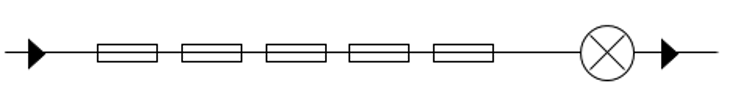
\includegraphics[width=10cm]{G1-Q43.png}\par}
	Với 5 cầu chỉ mắc nối tiếp trước một bóng đèn. Có nhiêu trường hợp dòng điện không thể truyền đến bóng đèn?
	\begin{enumerate}[label=\textbf{\Alph*.},align=left,left=1cm..0cm,itemindent=*]
	    \item 5 trường hợp. \item 120 trường hợp. \item 325 trường hợp. \item 31 trường hợp.
	\end{enumerate}
	\item Tìm số nguyên dương $n$ thỏa điều kiện $A_{n}^{2}-3C_{n}^{2}=15-5n$.
	\begin{enumerate}[label=\textbf{\Alph*.},align=left,left=1cm..0cm,itemindent=*]
	    \item $\left[ \begin{array}{l} n=5\\ n=6\\ n=12 \end{array} \right.$.
	    \item $\left[ \begin{array}{l} n=5\\ n=6 \end{array} \right.$.
	    \item $n=5$. \item $n=6$.
	\end{enumerate}
	\item Cần chọn ra một nhóm 3 người trong 7 người để tham gia lao động. Có bao nhiêu cách chọn?
	\begin{enumerate}[label=\textbf{\Alph*.},align=left,left=1cm..0cm,itemindent=*]
	    \item $210$. \item $21$. \item $10$. \item $35$.
	\end{enumerate}
\end{enumerate}\par

\noindent\textbf{Đáp án và các tham số:}
\begin{longtable}{|c|c|c|c|}\hline
	\textbf{Câu} & \textbf{Đáp án} & \textbf{Độ phân biệt ($a$)} & \textbf{Độ khó ($b$)} \\\hline
	\endhead
	1  & 4 & $2.93$ & $-0.09$ \\ \hline
	2  & 3 & $1.34$ & $-0.18$ \\ \hline
	3  & 3 & $1.69$ & $-0.31$ \\ \hline
	4  & 2 & $1.85$ & $-0.33$ \\ \hline
	5  & 2 & $1.4$  & $-0.6$  \\ \hline
	6  & 1 & $1.17$ & $-0.39$ \\ \hline
	7  & 4 & $0.96$ & $-0.81$ \\ \hline
	8  & 4 & $2.53$ & $0.31$  \\ \hline
	9  & 2 & $1.09$ & $-0.62$ \\ \hline
	10 & 4 & $0.89$ & $-1.33$ \\ \hline
\end{longtable}

\noindent\textbf{Câu hỏi trắc nghiệm phần Nhị thức Newton \cite{luyen2018xay}:}\par
\begin{enumerate}[label=\textbf{Câu \arabic*.},align=left,left=0cm..0cm,itemindent=*]
	% Nhị thức Newton
	\item (3.022) Cho khai triển $\left(x^3+2x^2+1\right)^{10}=a_1+a_2x+a_3x^2+...+a_{20}x^{20}$. Tính tổng $S=a_1+2a_2+4a_3+...+2^{20}a_{20}$.
	\begin{enumerate}[label=\textbf{\Alph*.},align=left,left=1cm..0cm,itemindent=*]
	    \item $S=15^{10}$. \item $S=17^{10}$. \item $S=17^{20}$. \item $S=7^{10}$.
	\end{enumerate}
	\item (3.068) Trong khai triển $(1-x)^{12}$, hệ số đứng trước $x^7$ là
	\begin{enumerate}[label=\textbf{\Alph*.},align=left,left=1cm..0cm,itemindent=*]
	    \item $330$. \item $-33$. \item $-72$. \item $-792$.
	\end{enumerate}
	\item (3.111) Công thức khai triển của $(a+b)^n$ là
	\begin{enumerate}[label=\textbf{\Alph*.},align=left,left=1cm..0cm,itemindent=*]
	    \item $\sum_{k=1}^nC_n^ka^{n+k}b^k$. \item $\sum_{k=0}^nC_n^ka^{n-k}b^k$. \item $\sum_{k=1}^nC_n^ka^{n-k}b^k$. \item $\sum_{k=0}^nC_n^ka^{n+k}b^k$.
	\end{enumerate}
	\item (3.112) Mệnh đề nào sau đây là đúng?
	\begin{enumerate}[label=\textbf{\Alph*.},align=left,left=1cm..0cm,itemindent=*]
	    \item $(a-b)^n=\sum_{k=0}^nC_n^ka^{n-k}b^k$, ($a,b\in\mathbb{R}$, $n\in\mathbb{N}^{*}$).
	    \item $(a-b)^n=\sum_{k=0}^n(-1)C_n^ka^{n-k}b^k$, ($a,b\in\mathbb{R}$, $n\in\mathbb{N}^{*}$).
	    \item $0^n=C_n^0+C_n^1+C_n^2+C_n^3+\ldots+C_n^n$, ($n\in\mathbb{N}^{*}$).
	    \item $2^n=C_n^0-C_n^1+C_n^2-C_n^3+\ldots+C_n^n$, ($n\in\mathbb{N}^{*}$).
	\end{enumerate}
	\item (3.113) Trong khai triển $(a+b)^n$, ($a,b\in\mathbb{R}$, $n\in\mathbb{N}^{*}$). Tổng các số mũ của $a$ và $b$ trong mỗi số hạng bằng
	\begin{enumerate}[label=\textbf{\Alph*.},align=left,left=1cm..0cm,itemindent=*]
	    \item $n+1$. \item $2n$. \item $n$. \item $2n+1$.
	\end{enumerate}
	\item (3.114) Trong khai triển $(a+b)^n$, ($a,b\in\mathbb{R}$, $n\in\mathbb{N}^{*}$), ta được bao nhiêu số hạng?
	\begin{enumerate}[label=\textbf{\Alph*.},align=left,left=1cm..0cm,itemindent=*]
	    \item $n+1$ số hạng. \item $2n$ số hạng. \item $n$ số hạng. \item $2n+1$ số hạng.
	\end{enumerate}
	\item (3.115) Số hạng tổng quát của khai triển $(a+b)^n$, ($a,b\in\mathbb{R}$, $n\in\mathbb{N}^{*}$) là
	\begin{enumerate}[label=\textbf{\Alph*.},align=left,left=1cm..0cm,itemindent=*]
	    \item $T_{k-1}=C_n^ka^{n-k}b^k$. \item $T_{k-1}=C_n^ka^{n+k}b^k$. \item $T_{k+1}=C_n^ka^{n-k}b^k$. \item $T_{k+1}=C_n^ka^{n+k}b^k$.
	\end{enumerate}
	\item (3.116) Tính tổng $S=2^{13}C_{13}^0-2^{12}.3^1C_{13}^1+2^{11}.3^2C_{13}^2-2^{10}.3^3C_{13}^3+...+3^{13}C_{13}^{13}$.
	\begin{enumerate}[label=\textbf{\Alph*.},align=left,left=1cm..0cm,itemindent=*]
	    \item $(-1)^{13}$. \item $5^{13}$. \item $(-5)^{13}$. \item $1^{13}$.
	\end{enumerate}
	\item (3.117) Nhị thức $(5+x^2)^{12}$ có khai triển là
	\begin{enumerate}[label=\textbf{\Alph*.},align=left,left=1cm..0cm,itemindent=*]
	    \item $5^{12}C_{12}^0-5^{11}xC_{12}^1+...+(-1)x^{24}C_{12}^{12}$.
	    \item $5^{12}C_{12}^0-5^{11}x^2C_{12}^1+...+ \left(-1\right) x^{24}C_{12}^{12}$.
	    \item $5^{12}C_{12}^0+5^{11}x^2C_{12}^1+...+x^{24}C_{12}^{12}$.
	    \item $5^{12}C_{12}^0+5^{11}xC_{12}^1+...+x^{24}C_{12}^{12}$.
	\end{enumerate}
	\item (3.118) Trong khai triển nhị thức $\left(x+y^2\right)^{10}$ thành đa thức và xếp theo thứ tự lũy thừa tăng dần của $x$ thì số hạng thứ 6 kể từ trái sang phải là bao nhiêu?
	\begin{enumerate}[label=\textbf{\Alph*.},align=left,left=1cm..0cm,itemindent=*]
	    \item $C_{10}^6x^4y^6$. \item $C_{10}^5x^5y^5$. \item $C_{10}^6x^4y^8$. \item $C_{10}^5x^5y^{10}$.
	\end{enumerate}
	\item (3.119) Trong khai triển $(2a-b)^5$, ($a,b\in\mathbb{R}$) hệ số của số hạng thứ 3 bằng
	\begin{enumerate}[label=\textbf{\Alph*.},align=left,left=1cm..0cm,itemindent=*]
	    \item $80$. \item $40$. \item $-80$. \item $-40$.
	\end{enumerate}
	\item (3.120) Khai triển nhị thức $(x+2)^{n+6}$, ($x\in\mathbb{R}$, $n\in\mathbb{N}$) có tất cả $17$ số hạng. Vậy $n$ bằng
	\begin{enumerate}[label=\textbf{\Alph*.},align=left,left=1cm..0cm,itemindent=*]
	    \item $10$. \item $11$. \item $12$. \item $17$.
	\end{enumerate}
	\item (3.121) Trong khai triển $\left(3x^2-y\right)^{10}$, hệ số của số hạng chính giữa là
	\begin{enumerate}[label=\textbf{\Alph*.},align=left,left=1cm..0cm,itemindent=*]
	    \item $-3^4C_{10}^4$. \item $3^4C_{10}^4$. \item $-3^5C_{10}^5$. \item $3^5C_{10}^5$.
	\end{enumerate}
	\item (3.122) Cho hàm số $f(x)=x(x+1)^{2018}$. Tính $f'(1)$.
	\begin{enumerate}[label=\textbf{\Alph*.},align=left,left=1cm..0cm,itemindent=*]
	    \item $f'(1)=2^{2018}+2^{2017}$.
	    \item $f'(1)=2^{2018}+2018.2^{2017}$.
	    \item $f'(1)=2^{2018}+2018.2^{2018}$.
	    \item $f'(1)=2^{2017}+2018.2^{2017}$.
	\end{enumerate}
	\item (3.123) Tìm số nguyên dương $n$ sao cho $C_n^0+2C_n^1+4C_n^2+...+2^nC_n^n=243$.
	\begin{enumerate}[label=\textbf{\Alph*.},align=left,left=1cm..0cm,itemindent=*]
	    \item $n=4$. \item $n=5$. \item $n=11$. \item $n=12$.
	\end{enumerate}
	\item (3.124) Cho khai triển $(2x-1)^4=a_0x^{14}+a_1x^{13}+...+a_{14}$. Tính tổng $T=a_0-a_1+a_2-a_3+...+a_{14}$.
	\begin{enumerate}[label=\textbf{\Alph*.},align=left,left=1cm..0cm,itemindent=*]
	    \item $T=1$. \item $T=3^4$. \item $T=-1$. \item $T=-3^4$.
	\end{enumerate}
	\item (3.125) Số nào sau đây không phải hệ số của $x^8$ trong khai triển $(1+x)^{10}$?
	\begin{enumerate}[label=\textbf{\Alph*.},align=left,left=1cm..0cm,itemindent=*]
	    \item $C_{10}^8-C_9^8$. \item $C_{10}^2$. \item $C_9^7+C_9^8$. \item $C_{10}^8$.
	\end{enumerate}
	\item (3.126) Cho khai triển $(x-2)^{100}=a_0+a_1x+a_2x^2+...+a_{100}x^{100}$. Hệ số $a_{97}$ là
	\begin{enumerate}[label=\textbf{\Alph*.},align=left,left=1cm..0cm,itemindent=*]
	    \item $-2^3C_{100}^3$. \item $-2^{97}C_{100}^{97}$. \item $2^3C_{100}^3$. \item $2^{97}C_{100}^{97}$.
	\end{enumerate}
	\item (3.127) Tìm giá trị nguyên dương $n$, biết $T=C_{2n}^0+C_{2n}^1+C_{2n}^2+...+C_{2n}^{2n}=1024$.
	\begin{enumerate}[label=\textbf{\Alph*.},align=left,left=1cm..0cm,itemindent=*]
	    \item $n=1$. \item $n=2$. \item $n=5$. \item $n=10$.
	\end{enumerate}
	\item (3.128) Tính tổng $S=n.3^0C_n^n+(n-1).3^1C_n^{n-1}+(n-2).3^2C_n^{n-2}+...+1.3^{n-1}C_n^1$.
	\begin{enumerate}[label=\textbf{\Alph*.},align=left,left=1cm..0cm,itemindent=*]
	    \item $S=n.4^{n-1}$. \item $S=n.4^n$. \item $S=n.3^n$. \item $S=n.3^{n-1}$.
	\end{enumerate}
	\item (3.129) Tìm số nguyên dương $n$ thỏa $$C_{2n-1}^1-2.2C_{2n-1}^2-3.2C_{2n-1}^3+...-(2n-1)x^{2n-2}C_{2n-1}^{2n-1}=2017.$$
	\begin{enumerate}[label=\textbf{\Alph*.},align=left,left=1cm..0cm,itemindent=*]
	    \item $n=1008$. \item $n=10009$. \item $n=-1008$. \item $n=-1009$.
	\end{enumerate}
	\item (3.130) Tìm hệ số lớn nhất của khai triển $(1+x)^n$. Biết rằng tổng tất cả các hệ số là $4096$.
	\begin{enumerate}[label=\textbf{\Alph*.},align=left,left=1cm..0cm,itemindent=*]
	    \item $0$. \item $1$. \item $C_{12}^5$. \item $C_{12}^6$.
	\end{enumerate}
	\item (3.131) Tính tổng $S=1.2^0C_{n+2}^1+2.2^1C_{n+2}^2+3.2^2C_{n+2}^3+...+(n+2).2^{n+1}C_{n+2}^{n+2}$.
	\begin{enumerate}[label=\textbf{\Alph*.},align=left,left=1cm..0cm,itemindent=*]
		\item $(n+2).3^{n+2}$. \item $(n+2).3^{n+1}$. \item $(n+2).2^{n+2}$. \item $(n+2).2^{n+1}$.
	\end{enumerate}
\end{enumerate}\par

\noindent\textbf{Đáp án và các tham số:}
\begin{longtable}{|c|c|c|c|}\hline
	\textbf{Câu} & \textbf{Đáp án} & \textbf{Độ phân biệt ($a$)} & \textbf{Độ khó ($b$)} \\\hline
	\endhead
	1 & B & $0.21$ & $0.00$ \\\hline
	2 & D & $1.74$ & $-1.28$ \\\hline
	3 & B & $1.31$ & $-1.18$ \\\hline
	4 & B & $0.36$ & $-1.73$ \\\hline
	5 & C & $0.78$ & $-0.67$ \\\hline
	6 & A & $0.53$ & $-2.09$ \\\hline
	7 & C & $0.81$ & $-1.34$ \\\hline
	8 & A & $1.26$ & $-0.40$ \\\hline
	9 & C & $0.17$ & $0.17$ \\\hline
	10 & D & $0.74$ & $-0.99$ \\\hline
	11 & A & $0.30$ & $0.41$ \\\hline
	12 & A & $1.57$ & $-0.94$ \\\hline
	13 & C & $1.06$ & $-0.98$ \\\hline
	14 & B & $1.28$ & $-1.49$ \\\hline
	15 & B & $0.33$ & $-2.25$ \\\hline
	16 & B & $0.29$ & $0.54$ \\\hline
	17 & A & $1.32$ & $-0.52$ \\\hline
	18 & A & $1.66$ & $-0.60$ \\\hline
	19 & C & $0.33$ & $0.48$ \\\hline
	20 & A & $0.50$ & $0.41$ \\\hline
	21 & C & $0.46$ & $0.90$ \\\hline
	22 & D & $0.37$ & $-0.61$ \\\hline
	23 & B & $0.17$ & $1.06$ \\\hline
\end{longtable}

\noindent\textbf{Câu hỏi trắc nghiệm phần Xác suất \cite{truc2018xay}:}
\begin{enumerate}[label=\textbf{Câu \arabic*.},align=left,left=0cm..0cm,itemindent=*]
	\item (4.028) Một nông dân có 8 con trâu. Hôm nay ông dắt theo 2 con để ra ruộng nhưng ông không biết rằng trong số trâu đó có 3 bị bệnh. Tính xác suất để cả 2 con trâu người nông dân chọn đều không bị bệnh.
	\begin{enumerate}[label=\textbf{\Alph*.},align=left,left=1cm..0cm,itemindent=*]
		\item $P=\frac 5{14}$. \item $P=\frac 5{28}$. \item $P=\frac{25}{28}$. \item $P=\frac 3{28}$.
	\end{enumerate}
	\item (4.030) Một khối lập phương có tất cả được sơn màu và được chia thành 125 khối nhỏ bằng nhau bởi các mặt phẳng song song với các mặt của khối lập phương (hình vẽ).\par
	{\centering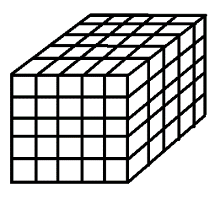
\includegraphics[width=4cm]{G2-Q30.png}\par}
	Lấy ngẫu nhiên 15 khối nhỏ. Xác suất để lấy được 6 khối nhỏ sơn đúng 1 mặt gần bằng
	\begin{enumerate}[label=\textbf{\Alph*.},align=left,left=1cm..0cm,itemindent=*]
		\item $0,00004$. \item $0,237$. \item $0,212$. \item $0,191$.
	\end{enumerate}
	\item (4.031) Lớp có 30 học sinh trong đó có 10 học sinh cận thị. Người ta lần lượt kiểm tra ngẫu nhiên từng học sinh cho đến khi phát hiện một học sinh cận thị thì dừng lại. Xác suất để kiểm tra tới học sinh thứ 5 thì ngừng lại (kiểm tra có hoàn lại) là
	\begin{enumerate}[label=\textbf{\Alph*.},align=left,left=1cm..0cm,itemindent=*]
		\item $0,068$. \item $0,067$. \item $0,066$. \item $0,065$.
	\end{enumerate}
	\item (4.040) Một lớp 30 học sinh. Chọn ngẫu nhiên 3 học sinh để tham gia hoạt động của Đoàn trường. Xác suất để chọn được 2 nam và 1 nữ là $\frac{54}{1015}$. Tính số học sinh nữ của lớp.
	\begin{enumerate}[label=\textbf{\Alph*.},align=left,left=1cm..0cm,itemindent=*]
		\item $18$. \item $15$. \item $12$. \item $9$.
	\end{enumerate}
	\item (4.055) Thả rơi một chất điểm vào một tấm bìa hình chữ nhật có chiều dài và chiều rộng lần lượt là 25 và 10 (cm). Một điểm $A$ cố định được vẽ trên tấm bìa như hình vẽ. Tính xác suất để chất điểm cách điểm $A$ từ 3 đến 4 (cm).\par
	{\centering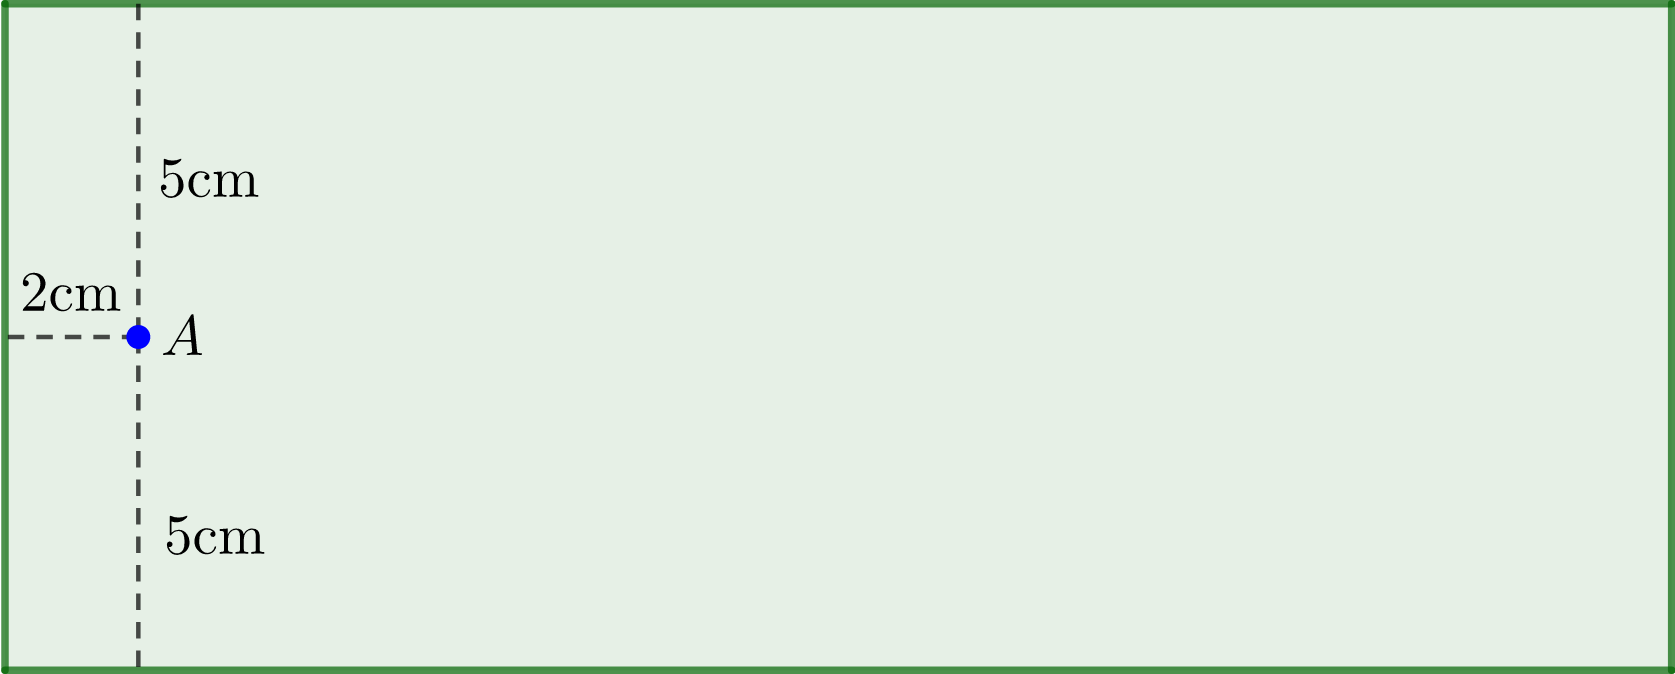
\includegraphics[width=8cm]{G2-Q58.png}\par}
	\begin{enumerate}[label=\textbf{\Alph*.},align=left,left=1cm..0cm,itemindent=*]
		\item $P=0,049$. \item $P=0,044$. \item $P=0,061$. \item $P=0,088$.
	\end{enumerate}
	\item (4.068) Ở người có một gen b gây bệnh bạch tạng lặn hoàn toàn so với gen B qui định màu da bình thường. Một đôi vợ chồng đều có gen đều dạng dị hợp (tức là có chứa một gen lặn). Tính xác suất để họ sinh được 5 đứa con thì 2 con trai bình thường, 2 con gái bình thường và 1 con trai bị bệnh.
	\begin{enumerate}[label=\textbf{\Alph*.},align=left,left=1cm..0cm,itemindent=*]
		\item $P=0,002$. \item $P=0,074$. \item $P=0,003$. \item $P=0,084$.
	\end{enumerate}
	\item (4.083) Lỗi chính tả của một học sinh lớp 2 trên mỗi trang vở là đại lượng ngẫu nhiên $X$ có bảng phân phối xác suất như sau:
	\begin{longtable}{|c|c|c|c|c|c|c|}\hline
	$X$ & 0   & 1   & 2   & 3    & 4    & 5   \\ \hline
	$P$ & 0,3 & 0,3 & 0,2 & 0,01 & 0,09 & 0,1 \\ \hline
	\end{longtable}
	Tính xác suất để mỗi trang sai ít nhất 3 lỗi.
	\begin{enumerate}[label=\textbf{\Alph*.},align=left,left=1cm..0cm,itemindent=*]
		\item $P=0,2$. \item $P=0,3$. \item $P=0,29$. \item $P=0,009$.
	\end{enumerate}
	\item (4.087) Lợi nhuận (tỷ đồng) hai dự án $A$ và $B$, ký hiệu $X_A$ và $X_B$ có bảng phân phối xác suất như sau:
	\begin{longtable}{|c|c|c|c|}\hline
	$X_A$ & $-2$ & 3   & 10  \\ \hline
	$P$   & 0.2  & 0.6 & 0.2 \\ \hline\hline
	$X_B$ & 1    & 4   & 9   \\ \hline
	$P$   & 0.4  & 0.4 & 0.2 \\ \hline
	\end{longtable}
	Tìm lợi nhuận trung bình của mỗi dự án và dự án nào có độ ổn định cao hơn?
	\begin{enumerate}[label=\textbf{\Alph*.},align=left,left=1cm..0cm,itemindent=*]
		\item $E\left( {{X}_{A}} \right)=3,4; E\left( {{X}_{B}} \right)=3,3$ và dự án $A$ ổn định hơn.
		\item $E\left( {{X}_{A}} \right)=3,4; E\left( {{X}_{B}} \right)=3,3$ và dự án $B$ ổn định hơn.
		\item $E\left( {{X}_{A}} \right)=3,3; E\left( {{X}_{B}} \right)=3,4$ và dự án $A$ ổn định hơn.
		\item $E\left( {{X}_{A}} \right)=3,3; E\left( {{X}_{B}} \right)=3,4$ và dự án $B$ ổn định hơn.
	\end{enumerate}
	\item (4.123) Khảo sát trên 100 sinh viên về thời gian sử dụng máy tính trong một ngày thu được biểu đồ sau:\par
	{\centering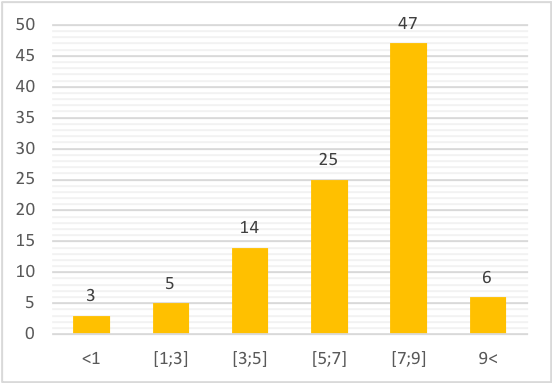
\includegraphics[width=7cm]{G2-Q127.png}\par}
	Gọi $X$ là đại lượng thời gian sử dụng máy tính (giờ). Tính $P\left( 5,28\leqslant X<9 \right)$.
	\begin{enumerate}[label=\textbf{\Alph*.},align=left,left=1cm..0cm,itemindent=*]
		\item $P\left( 5,28\leqslant X<9,2 \right)=0,78$.
		\item $P\left( 5,28\leqslant X<9,2 \right)=0,47$.
		\item $P\left( 5,28\leqslant X<9,2 \right)=0,72$.
		\item $P\left( 5,28\leqslant X<9,2 \right)=0,53$.
	\end{enumerate}
	\item (4.127) Một người đi bộ từ công ty về đến nhà thì phát hiện rớt mất ví tiền. Anh ta chắc chắn rằng ví bị rơi trên đoạn đường khoảng 100m trước cửa công ty nên quay lại tìm. Tính xác suất anh ta tìm được ví biết quãng đường từ nhà đến công ty là 1,5km.
	\begin{enumerate}[label=\textbf{\Alph*.},align=left,left=1cm..0cm,itemindent=*]
		\item $P=\frac 1{15}$. \item $P=\frac 3{200}$. \item $P=\frac {14}{15}$. \item $P=\frac 16$.
	\end{enumerate}
	\item (4.128) Số lượng cá (kg) một ngư dân bắt được mỗi ngày được thống kê trong bảng sau:
	\begin{longtable}{|l|c|c|c|c|c|c|}\hline
	$X$ (kg) & 0     & 1      & 2    & 3      & 4      & 5     \\ \hline
	Xác suất & 1,6\% & 12,6\% & 21\% & 34,7\% & 21,9\% & 8,2\% \\ \hline
	\end{longtable}
	Tính xác suất để người này câu được nhiều nhất 2kg cá.
	\begin{enumerate}[label=\textbf{\Alph*.},align=left,left=1cm..0cm,itemindent=*]
		\item $P=0,04\%$. \item $P=35,2\%$. \item $P=0,21\%$. \item $P=0,352\%$.
	\end{enumerate}
\end{enumerate}\par

% \section{Xây dựng API tạo đề kiểm tra}
% Với các ứng dụng không cùng nền tảng, ta cần một \textit{giao thức} (Application programming interface – API) để trao đổi thông tin giữa các bên\cite{tuan2020mobile}.

\section{Xây dựng API xử lý dữ liệu}
